% id: 24-18
% book: 100발100중 3-2 중간 · 01 3-2 중간(삼각비·삼각비의 활용·원과 직선·원주각·부록)
% section: 실전 문제 1회
% figure: crop:fig-24-18-2.png
% answer: ②
% answer_source: 답지(빠른정답)
% variant_level: 0 (원본 전사)
% 이 파일은 build.mjs 가 items.json 에서 만든다. 고칠 때는 items.json 을 고친다.
\smash{\raisebox{1.5mm}{\dmkichul{100발100중 3-2 중간 24쪽 18번}}}
\noindent\begin{minipage}[t]{0.58\linewidth}\vspace{0pt}\raggedright 그림과 같은 직각삼각형~$\pt{ABC}$에서 $x$의 값을 주어진 삼각비의 표를 이용하여 구하면?\end{minipage}\hfill\begin{minipage}[t]{0.4\linewidth}\vspace{0pt}\centering 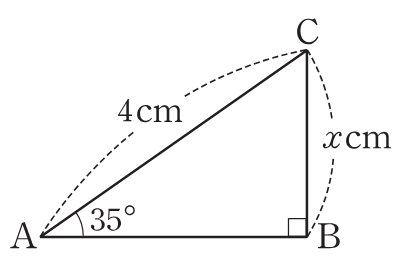
\includegraphics[width=95.9pt]{figures/fig-24-18-2.png}\end{minipage}\par
\par\smallskip\begin{center}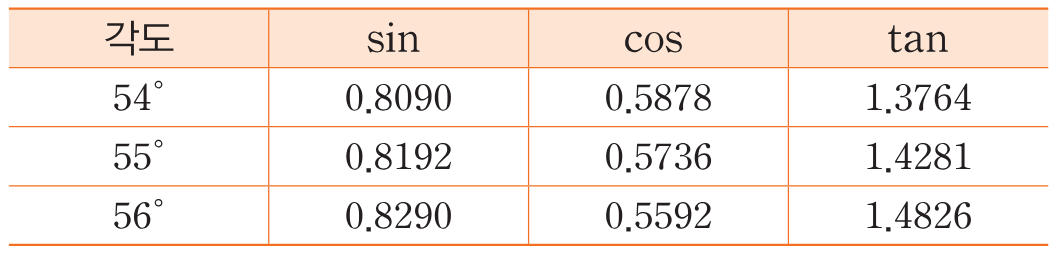
\includegraphics[width=253.4pt]{figures/fig-24-18.png}\end{center}
\begin{choices32}{$1.4281$}{$2.2944$}{$3.2768$}{$5.5056$}{$5.7124$}\end{choices32}
